\usetikzlibrary{arrows.meta}
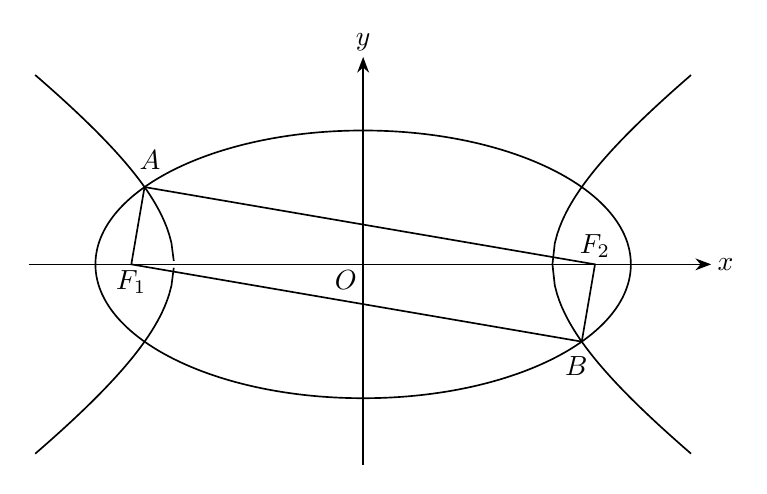
\begin{tikzpicture}[x=1.7cm,y=1.7cm,line width=.6pt,font=\normalsize,>=Stealth]
  \coordinate (F1) at (-1.7320508,0);
  \coordinate (F2) at (1.7320508,0);
  \coordinate (A) at (-1.6329932,0.5773503);
  \coordinate (B) at (1.6329932,-0.5773503);
  \draw[->] (-2.5,0) -- (2.6,0) node[right,inner sep=2pt] {$x$};
  \draw[->] (0,-1.5) -- (0,1.55) node[above,inner sep=2pt] {$y$};
  \node[below left,inner sep=2pt] at (0,0) {$O$};
  \draw (0,0) ellipse[x radius=2,y radius=1];
  \draw[domain=-2.45:-1.4142136,samples=60] plot (\x,{sqrt(\x*\x/2-1)});
  \draw[domain=-2.45:-1.4142136,samples=60] plot (\x,{-sqrt(\x*\x/2-1)});
  \draw[domain=1.4142136:2.45,samples=60] plot (\x,{sqrt(\x*\x/2-1)});
  \draw[domain=1.4142136:2.45,samples=60] plot (\x,{-sqrt(\x*\x/2-1)});
  \draw (A)--(F1)--(B)--(F2)--cycle;
  \node[above,yshift=4pt,xshift=2pt,inner sep=2pt] at (A) {$A$};
  \node[below,inner sep=2pt] at (F1) {$F_1$};
  \node[above,inner sep=2pt] at (F2) {$F_2$};
  \node[below,yshift=-3pt,xshift=-2pt,inner sep=2pt] at (B) {$B$};
\end{tikzpicture}
